% Graphic for TeX using PGF
% Title: /home/tomgli/workspace/github.com/bachopp/thesis/files/chapters/background/graphs/modelflux.dia
% Creator: Dia v0.97.3
% CreationDate: Mon May 16 20:32:13 2016
% For: tomgli
% \usepackage{tikz}
% The following commands are not supported in PSTricks at present
% We define them conditionally, so when they are implemented,
% this pgf file will use them.
\ifx\du\undefined
  \newlength{\du}
\fi
\setlength{\du}{15\unitlength}
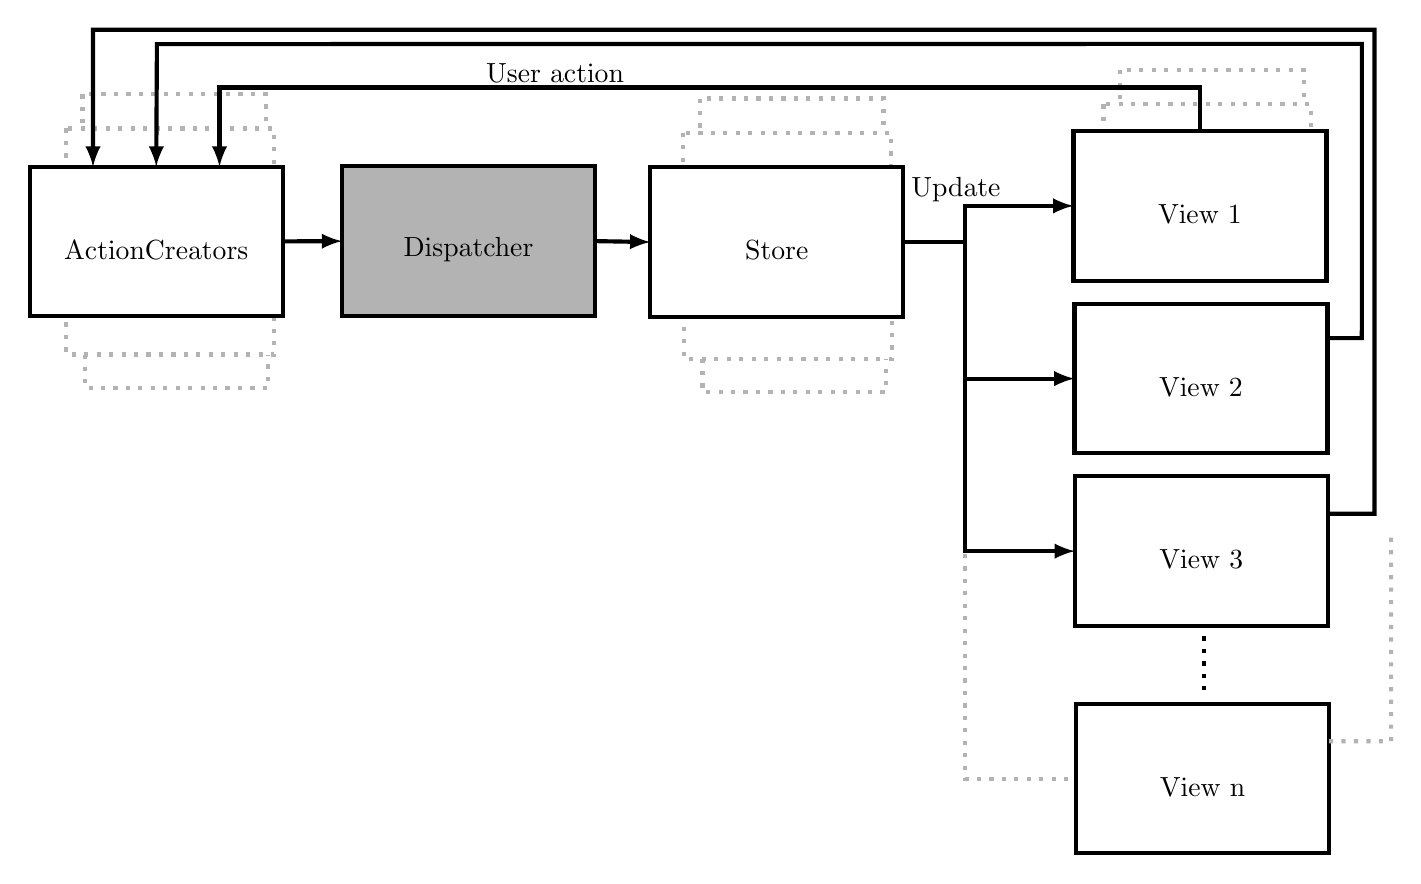
\begin{tikzpicture}
\pgftransformxscale{1.000000}
\pgftransformyscale{-1.000000}
\definecolor{dialinecolor}{rgb}{0.000000, 0.000000, 0.000000}
\pgfsetstrokecolor{dialinecolor}
\definecolor{dialinecolor}{rgb}{1.000000, 1.000000, 1.000000}
\pgfsetfillcolor{dialinecolor}
\definecolor{dialinecolor}{rgb}{1.000000, 1.000000, 1.000000}
\pgfsetfillcolor{dialinecolor}
\fill (5.095014\du,8.490457\du)--(5.095014\du,10.503187\du)--(9.510453\du,10.503187\du)--(9.510453\du,8.490457\du)--cycle;
\pgfsetlinewidth{0.100000\du}
\pgfsetdash{{\pgflinewidth}{0.200000\du}}{0cm}
\pgfsetdash{{\pgflinewidth}{0.200000\du}}{0cm}
\pgfsetmiterjoin
\definecolor{dialinecolor}{rgb}{0.701961, 0.701961, 0.701961}
\pgfsetstrokecolor{dialinecolor}
\draw (5.095014\du,8.490457\du)--(5.095014\du,10.503187\du)--(9.510453\du,10.503187\du)--(9.510453\du,8.490457\du)--cycle;
% setfont left to latex
\definecolor{dialinecolor}{rgb}{0.000000, 0.000000, 0.000000}
\pgfsetstrokecolor{dialinecolor}
\node at (7.302733\du,9.696822\du){};
\definecolor{dialinecolor}{rgb}{1.000000, 1.000000, 1.000000}
\pgfsetfillcolor{dialinecolor}
\fill (5.038646\du,3.426908\du)--(5.038646\du,5.439638\du)--(9.454086\du,5.439638\du)--(9.454086\du,3.426908\du)--cycle;
\pgfsetlinewidth{0.100000\du}
\pgfsetdash{{\pgflinewidth}{0.200000\du}}{0cm}
\pgfsetdash{{\pgflinewidth}{0.200000\du}}{0cm}
\pgfsetmiterjoin
\definecolor{dialinecolor}{rgb}{0.701961, 0.701961, 0.701961}
\pgfsetstrokecolor{dialinecolor}
\draw (5.038646\du,3.426908\du)--(5.038646\du,5.439638\du)--(9.454086\du,5.439638\du)--(9.454086\du,3.426908\du)--cycle;
% setfont left to latex
\definecolor{dialinecolor}{rgb}{0.000000, 0.000000, 0.000000}
\pgfsetstrokecolor{dialinecolor}
\node at (7.246366\du,4.633273\du){};
\definecolor{dialinecolor}{rgb}{1.000000, 1.000000, 1.000000}
\pgfsetfillcolor{dialinecolor}
\fill (4.632653\du,4.247344\du)--(4.632653\du,6.519266\du)--(9.642692\du,6.519266\du)--(9.642692\du,4.247344\du)--cycle;
\pgfsetlinewidth{0.100000\du}
\pgfsetdash{{\pgflinewidth}{0.200000\du}}{0cm}
\pgfsetdash{{\pgflinewidth}{0.200000\du}}{0cm}
\pgfsetmiterjoin
\definecolor{dialinecolor}{rgb}{0.701961, 0.701961, 0.701961}
\pgfsetstrokecolor{dialinecolor}
\draw (4.632653\du,4.247344\du)--(4.632653\du,6.519266\du)--(9.642692\du,6.519266\du)--(9.642692\du,4.247344\du)--cycle;
% setfont left to latex
\definecolor{dialinecolor}{rgb}{0.000000, 0.000000, 0.000000}
\pgfsetstrokecolor{dialinecolor}
\node at (7.137673\du,5.583305\du){};
\definecolor{dialinecolor}{rgb}{1.000000, 1.000000, 1.000000}
\pgfsetfillcolor{dialinecolor}
\fill (4.650331\du,7.421637\du)--(4.650331\du,9.693559\du)--(9.660370\du,9.693559\du)--(9.660370\du,7.421637\du)--cycle;
\pgfsetlinewidth{0.100000\du}
\pgfsetdash{{\pgflinewidth}{0.200000\du}}{0cm}
\pgfsetdash{{\pgflinewidth}{0.200000\du}}{0cm}
\pgfsetmiterjoin
\definecolor{dialinecolor}{rgb}{0.701961, 0.701961, 0.701961}
\pgfsetstrokecolor{dialinecolor}
\draw (4.650331\du,7.421637\du)--(4.650331\du,9.693559\du)--(9.660370\du,9.693559\du)--(9.660370\du,7.421637\du)--cycle;
% setfont left to latex
\definecolor{dialinecolor}{rgb}{0.000000, 0.000000, 0.000000}
\pgfsetstrokecolor{dialinecolor}
\node at (7.155350\du,8.757598\du){};
\definecolor{dialinecolor}{rgb}{1.000000, 1.000000, 1.000000}
\pgfsetfillcolor{dialinecolor}
\fill (19.973079\du,8.590730\du)--(19.973079\du,10.603460\du)--(24.388519\du,10.603460\du)--(24.388519\du,8.590730\du)--cycle;
\pgfsetlinewidth{0.100000\du}
\pgfsetdash{{\pgflinewidth}{0.200000\du}}{0cm}
\pgfsetdash{{\pgflinewidth}{0.200000\du}}{0cm}
\pgfsetmiterjoin
\definecolor{dialinecolor}{rgb}{0.701961, 0.701961, 0.701961}
\pgfsetstrokecolor{dialinecolor}
\draw (19.973079\du,8.590730\du)--(19.973079\du,10.603460\du)--(24.388519\du,10.603460\du)--(24.388519\du,8.590730\du)--cycle;
% setfont left to latex
\definecolor{dialinecolor}{rgb}{0.000000, 0.000000, 0.000000}
\pgfsetstrokecolor{dialinecolor}
\node at (22.180799\du,9.797095\du){};
\definecolor{dialinecolor}{rgb}{1.000000, 1.000000, 1.000000}
\pgfsetfillcolor{dialinecolor}
\fill (19.916712\du,3.527181\du)--(19.916712\du,5.539911\du)--(24.332152\du,5.539911\du)--(24.332152\du,3.527181\du)--cycle;
\pgfsetlinewidth{0.100000\du}
\pgfsetdash{{\pgflinewidth}{0.200000\du}}{0cm}
\pgfsetdash{{\pgflinewidth}{0.200000\du}}{0cm}
\pgfsetmiterjoin
\definecolor{dialinecolor}{rgb}{0.701961, 0.701961, 0.701961}
\pgfsetstrokecolor{dialinecolor}
\draw (19.916712\du,3.527181\du)--(19.916712\du,5.539911\du)--(24.332152\du,5.539911\du)--(24.332152\du,3.527181\du)--cycle;
% setfont left to latex
\definecolor{dialinecolor}{rgb}{0.000000, 0.000000, 0.000000}
\pgfsetstrokecolor{dialinecolor}
\node at (22.124432\du,4.733546\du){};
\definecolor{dialinecolor}{rgb}{1.000000, 1.000000, 1.000000}
\pgfsetfillcolor{dialinecolor}
\fill (19.510719\du,4.347617\du)--(19.510719\du,6.619539\du)--(24.520758\du,6.619539\du)--(24.520758\du,4.347617\du)--cycle;
\pgfsetlinewidth{0.100000\du}
\pgfsetdash{{\pgflinewidth}{0.200000\du}}{0cm}
\pgfsetdash{{\pgflinewidth}{0.200000\du}}{0cm}
\pgfsetmiterjoin
\definecolor{dialinecolor}{rgb}{0.701961, 0.701961, 0.701961}
\pgfsetstrokecolor{dialinecolor}
\draw (19.510719\du,4.347617\du)--(19.510719\du,6.619539\du)--(24.520758\du,6.619539\du)--(24.520758\du,4.347617\du)--cycle;
% setfont left to latex
\definecolor{dialinecolor}{rgb}{0.000000, 0.000000, 0.000000}
\pgfsetstrokecolor{dialinecolor}
\node at (22.015738\du,5.683578\du){};
\definecolor{dialinecolor}{rgb}{1.000000, 1.000000, 1.000000}
\pgfsetfillcolor{dialinecolor}
\fill (19.528396\du,7.521910\du)--(19.528396\du,9.793832\du)--(24.538435\du,9.793832\du)--(24.538435\du,7.521910\du)--cycle;
\pgfsetlinewidth{0.100000\du}
\pgfsetdash{{\pgflinewidth}{0.200000\du}}{0cm}
\pgfsetdash{{\pgflinewidth}{0.200000\du}}{0cm}
\pgfsetmiterjoin
\definecolor{dialinecolor}{rgb}{0.701961, 0.701961, 0.701961}
\pgfsetstrokecolor{dialinecolor}
\draw (19.528396\du,7.521910\du)--(19.528396\du,9.793832\du)--(24.538435\du,9.793832\du)--(24.538435\du,7.521910\du)--cycle;
% setfont left to latex
\definecolor{dialinecolor}{rgb}{0.000000, 0.000000, 0.000000}
\pgfsetstrokecolor{dialinecolor}
\node at (22.033416\du,8.857871\du){};
\definecolor{dialinecolor}{rgb}{1.000000, 1.000000, 1.000000}
\pgfsetfillcolor{dialinecolor}
\fill (30.037803\du,2.846602\du)--(30.037803\du,4.859332\du)--(34.453243\du,4.859332\du)--(34.453243\du,2.846602\du)--cycle;
\pgfsetlinewidth{0.100000\du}
\pgfsetdash{{\pgflinewidth}{0.200000\du}}{0cm}
\pgfsetdash{{\pgflinewidth}{0.200000\du}}{0cm}
\pgfsetmiterjoin
\definecolor{dialinecolor}{rgb}{0.701961, 0.701961, 0.701961}
\pgfsetstrokecolor{dialinecolor}
\draw (30.037803\du,2.846602\du)--(30.037803\du,4.859332\du)--(34.453243\du,4.859332\du)--(34.453243\du,2.846602\du)--cycle;
% setfont left to latex
\definecolor{dialinecolor}{rgb}{0.000000, 0.000000, 0.000000}
\pgfsetstrokecolor{dialinecolor}
\node at (32.245523\du,4.052967\du){};
\definecolor{dialinecolor}{rgb}{1.000000, 1.000000, 1.000000}
\pgfsetfillcolor{dialinecolor}
\fill (29.631810\du,3.667038\du)--(29.631810\du,5.938960\du)--(34.641849\du,5.938960\du)--(34.641849\du,3.667038\du)--cycle;
\pgfsetlinewidth{0.100000\du}
\pgfsetdash{{\pgflinewidth}{0.200000\du}}{0cm}
\pgfsetdash{{\pgflinewidth}{0.200000\du}}{0cm}
\pgfsetmiterjoin
\definecolor{dialinecolor}{rgb}{0.701961, 0.701961, 0.701961}
\pgfsetstrokecolor{dialinecolor}
\draw (29.631810\du,3.667038\du)--(29.631810\du,5.938960\du)--(34.641849\du,5.938960\du)--(34.641849\du,3.667038\du)--cycle;
% setfont left to latex
\definecolor{dialinecolor}{rgb}{0.000000, 0.000000, 0.000000}
\pgfsetstrokecolor{dialinecolor}
\node at (32.136830\du,5.002999\du){};
\pgfsetlinewidth{0.100000\du}
\pgfsetdash{{\pgflinewidth}{0.200000\du}}{0cm}
\pgfsetdash{{\pgflinewidth}{0.200000\du}}{0cm}
\pgfsetmiterjoin
\pgfsetbuttcap
{
\definecolor{dialinecolor}{rgb}{0.701961, 0.701961, 0.701961}
\pgfsetfillcolor{dialinecolor}
% was here!!!
{\pgfsetcornersarced{\pgfpoint{0.000000\du}{0.000000\du}}\definecolor{dialinecolor}{rgb}{0.701961, 0.701961, 0.701961}
\pgfsetstrokecolor{dialinecolor}
\draw (24.810173\du,6.984146\du)--(26.297571\du,6.984146\du)--(26.297571\du,19.909119\du)--(28.971295\du,19.909119\du);
}}
\definecolor{dialinecolor}{rgb}{1.000000, 1.000000, 1.000000}
\pgfsetfillcolor{dialinecolor}
\fill (28.908980\du,4.311671\du)--(28.908980\du,7.913062\du)--(35.003653\du,7.913062\du)--(35.003653\du,4.311671\du)--cycle;
\pgfsetlinewidth{0.100000\du}
\pgfsetdash{}{0pt}
\pgfsetdash{}{0pt}
\pgfsetmiterjoin
\definecolor{dialinecolor}{rgb}{0.000000, 0.000000, 0.000000}
\pgfsetstrokecolor{dialinecolor}
\draw (28.908980\du,4.311671\du)--(28.908980\du,7.913062\du)--(35.003653\du,7.913062\du)--(35.003653\du,4.311671\du)--cycle;
% setfont left to latex
\definecolor{dialinecolor}{rgb}{0.000000, 0.000000, 0.000000}
\pgfsetstrokecolor{dialinecolor}
\node at (31.956317\du,6.312367\du){View 1};
\definecolor{dialinecolor}{rgb}{1.000000, 1.000000, 1.000000}
\pgfsetfillcolor{dialinecolor}
\fill (3.767030\du,5.167300\du)--(3.767030\du,8.768692\du)--(9.861703\du,8.768692\du)--(9.861703\du,5.167300\du)--cycle;
\pgfsetlinewidth{0.100000\du}
\pgfsetdash{}{0pt}
\pgfsetdash{}{0pt}
\pgfsetmiterjoin
\definecolor{dialinecolor}{rgb}{0.000000, 0.000000, 0.000000}
\pgfsetstrokecolor{dialinecolor}
\draw (3.767030\du,5.167300\du)--(3.767030\du,8.768692\du)--(9.861703\du,8.768692\du)--(9.861703\du,5.167300\du)--cycle;
% setfont left to latex
\definecolor{dialinecolor}{rgb}{0.000000, 0.000000, 0.000000}
\pgfsetstrokecolor{dialinecolor}
\node at (6.814366\du,7.167996\du){ActionCreators};
\definecolor{dialinecolor}{rgb}{0.701961, 0.701961, 0.701961}
\pgfsetfillcolor{dialinecolor}
\fill (11.288700\du,5.160520\du)--(11.288700\du,8.761912\du)--(17.383373\du,8.761912\du)--(17.383373\du,5.160520\du)--cycle;
\pgfsetlinewidth{0.100000\du}
\pgfsetdash{}{0pt}
\pgfsetdash{}{0pt}
\pgfsetmiterjoin
\definecolor{dialinecolor}{rgb}{0.000000, 0.000000, 0.000000}
\pgfsetstrokecolor{dialinecolor}
\draw (11.288700\du,5.160520\du)--(11.288700\du,8.761912\du)--(17.383373\du,8.761912\du)--(17.383373\du,5.160520\du)--cycle;
% setfont left to latex
\definecolor{dialinecolor}{rgb}{0.000000, 0.000000, 0.000000}
\pgfsetstrokecolor{dialinecolor}
\node at (14.336036\du,7.161216\du){Dispatcher};
\definecolor{dialinecolor}{rgb}{1.000000, 1.000000, 1.000000}
\pgfsetfillcolor{dialinecolor}
\fill (18.715500\du,5.183450\du)--(18.715500\du,8.784842\du)--(24.810173\du,8.784842\du)--(24.810173\du,5.183450\du)--cycle;
\pgfsetlinewidth{0.100000\du}
\pgfsetdash{}{0pt}
\pgfsetdash{}{0pt}
\pgfsetmiterjoin
\definecolor{dialinecolor}{rgb}{0.000000, 0.000000, 0.000000}
\pgfsetstrokecolor{dialinecolor}
\draw (18.715500\du,5.183450\du)--(18.715500\du,8.784842\du)--(24.810173\du,8.784842\du)--(24.810173\du,5.183450\du)--cycle;
% setfont left to latex
\definecolor{dialinecolor}{rgb}{0.000000, 0.000000, 0.000000}
\pgfsetstrokecolor{dialinecolor}
\node at (21.762836\du,7.184146\du){Store};
\pgfsetlinewidth{0.100000\du}
\pgfsetdash{}{0pt}
\pgfsetdash{}{0pt}
\pgfsetbuttcap
{
\definecolor{dialinecolor}{rgb}{0.000000, 0.000000, 0.000000}
\pgfsetfillcolor{dialinecolor}
% was here!!!
\pgfsetarrowsend{latex}
\definecolor{dialinecolor}{rgb}{0.000000, 0.000000, 0.000000}
\pgfsetstrokecolor{dialinecolor}
\draw (9.861703\du,6.967996\du)--(11.288700\du,6.961216\du);
}
\pgfsetlinewidth{0.100000\du}
\pgfsetdash{}{0pt}
\pgfsetdash{}{0pt}
\pgfsetbuttcap
{
\definecolor{dialinecolor}{rgb}{0.000000, 0.000000, 0.000000}
\pgfsetfillcolor{dialinecolor}
% was here!!!
\pgfsetarrowsend{latex}
\definecolor{dialinecolor}{rgb}{0.000000, 0.000000, 0.000000}
\pgfsetstrokecolor{dialinecolor}
\draw (17.383373\du,6.961216\du)--(18.715500\du,6.984146\du);
}
\pgfsetlinewidth{0.100000\du}
\pgfsetdash{}{0pt}
\pgfsetdash{}{0pt}
\pgfsetmiterjoin
\pgfsetbuttcap
{
\definecolor{dialinecolor}{rgb}{0.000000, 0.000000, 0.000000}
\pgfsetfillcolor{dialinecolor}
% was here!!!
\pgfsetarrowsend{latex}
{\pgfsetcornersarced{\pgfpoint{0.000000\du}{0.000000\du}}\definecolor{dialinecolor}{rgb}{0.000000, 0.000000, 0.000000}
\pgfsetstrokecolor{dialinecolor}
\draw (31.956317\du,4.311671\du)--(31.956317\du,3.261671\du)--(8.338035\du,3.261671\du)--(8.338035\du,5.167300\du);
}}
% setfont left to latex
\definecolor{dialinecolor}{rgb}{0.000000, 0.000000, 0.000000}
\pgfsetstrokecolor{dialinecolor}
\node at (16.420910\du,2.917064\du){User action};
% setfont left to latex
\definecolor{dialinecolor}{rgb}{0.000000, 0.000000, 0.000000}
\pgfsetstrokecolor{dialinecolor}
\node at (26.077199\du,5.718444\du){Update};
\definecolor{dialinecolor}{rgb}{1.000000, 1.000000, 1.000000}
\pgfsetfillcolor{dialinecolor}
\fill (28.933238\du,8.472621\du)--(28.933238\du,12.074012\du)--(35.027911\du,12.074012\du)--(35.027911\du,8.472621\du)--cycle;
\pgfsetlinewidth{0.100000\du}
\pgfsetdash{}{0pt}
\pgfsetdash{}{0pt}
\pgfsetmiterjoin
\definecolor{dialinecolor}{rgb}{0.000000, 0.000000, 0.000000}
\pgfsetstrokecolor{dialinecolor}
\draw (28.933238\du,8.472621\du)--(28.933238\du,12.074012\du)--(35.027911\du,12.074012\du)--(35.027911\du,8.472621\du)--cycle;
% setfont left to latex
\definecolor{dialinecolor}{rgb}{0.000000, 0.000000, 0.000000}
\pgfsetstrokecolor{dialinecolor}
\node at (31.980575\du,10.473317\du){View 2};
\definecolor{dialinecolor}{rgb}{1.000000, 1.000000, 1.000000}
\pgfsetfillcolor{dialinecolor}
\fill (28.943205\du,12.628736\du)--(28.943205\du,16.230128\du)--(35.037877\du,16.230128\du)--(35.037877\du,12.628736\du)--cycle;
\pgfsetlinewidth{0.100000\du}
\pgfsetdash{}{0pt}
\pgfsetdash{}{0pt}
\pgfsetmiterjoin
\definecolor{dialinecolor}{rgb}{0.000000, 0.000000, 0.000000}
\pgfsetstrokecolor{dialinecolor}
\draw (28.943205\du,12.628736\du)--(28.943205\du,16.230128\du)--(35.037877\du,16.230128\du)--(35.037877\du,12.628736\du)--cycle;
% setfont left to latex
\definecolor{dialinecolor}{rgb}{0.000000, 0.000000, 0.000000}
\pgfsetstrokecolor{dialinecolor}
\node at (31.990541\du,14.629432\du){View 3};
\pgfsetlinewidth{0.100000\du}
\pgfsetdash{}{0pt}
\pgfsetdash{}{0pt}
\pgfsetmiterjoin
\pgfsetbuttcap
{
\definecolor{dialinecolor}{rgb}{0.000000, 0.000000, 0.000000}
\pgfsetfillcolor{dialinecolor}
% was here!!!
\pgfsetarrowsend{latex}
{\pgfsetcornersarced{\pgfpoint{0.000000\du}{0.000000\du}}\definecolor{dialinecolor}{rgb}{0.000000, 0.000000, 0.000000}
\pgfsetstrokecolor{dialinecolor}
\draw (24.810173\du,6.984146\du)--(26.302849\du,6.984146\du)--(26.302849\du,6.112367\du)--(28.908980\du,6.112367\du);
}}
\pgfsetlinewidth{0.100000\du}
\pgfsetdash{}{0pt}
\pgfsetdash{}{0pt}
\pgfsetmiterjoin
\pgfsetbuttcap
{
\definecolor{dialinecolor}{rgb}{0.000000, 0.000000, 0.000000}
\pgfsetfillcolor{dialinecolor}
% was here!!!
\pgfsetarrowsend{latex}
{\pgfsetcornersarced{\pgfpoint{0.000000\du}{0.000000\du}}\definecolor{dialinecolor}{rgb}{0.000000, 0.000000, 0.000000}
\pgfsetstrokecolor{dialinecolor}
\draw (24.810173\du,6.984146\du)--(26.306447\du,6.984146\du)--(26.306447\du,10.273317\du)--(28.933238\du,10.273317\du);
}}
\pgfsetlinewidth{0.100000\du}
\pgfsetdash{}{0pt}
\pgfsetdash{}{0pt}
\pgfsetmiterjoin
\pgfsetbuttcap
{
\definecolor{dialinecolor}{rgb}{0.000000, 0.000000, 0.000000}
\pgfsetfillcolor{dialinecolor}
% was here!!!
\pgfsetarrowsend{latex}
{\pgfsetcornersarced{\pgfpoint{0.000000\du}{0.000000\du}}\definecolor{dialinecolor}{rgb}{0.000000, 0.000000, 0.000000}
\pgfsetstrokecolor{dialinecolor}
\draw (24.810173\du,6.984146\du)--(26.302849\du,6.984146\du)--(26.302849\du,14.429432\du)--(28.943205\du,14.429432\du);
}}
\definecolor{dialinecolor}{rgb}{1.000000, 1.000000, 1.000000}
\pgfsetfillcolor{dialinecolor}
\fill (28.971295\du,18.108423\du)--(28.971295\du,21.709814\du)--(35.065968\du,21.709814\du)--(35.065968\du,18.108423\du)--cycle;
\pgfsetlinewidth{0.100000\du}
\pgfsetdash{}{0pt}
\pgfsetdash{}{0pt}
\pgfsetmiterjoin
\definecolor{dialinecolor}{rgb}{0.000000, 0.000000, 0.000000}
\pgfsetstrokecolor{dialinecolor}
\draw (28.971295\du,18.108423\du)--(28.971295\du,21.709814\du)--(35.065968\du,21.709814\du)--(35.065968\du,18.108423\du)--cycle;
% setfont left to latex
\definecolor{dialinecolor}{rgb}{0.000000, 0.000000, 0.000000}
\pgfsetstrokecolor{dialinecolor}
\node at (32.018631\du,20.109119\du){View n};
\pgfsetlinewidth{0.100000\du}
\pgfsetdash{{\pgflinewidth}{0.200000\du}}{0cm}
\pgfsetdash{{\pgflinewidth}{0.200000\du}}{0cm}
\pgfsetbuttcap
{
\definecolor{dialinecolor}{rgb}{0.000000, 0.000000, 0.000000}
\pgfsetfillcolor{dialinecolor}
% was here!!!
\definecolor{dialinecolor}{rgb}{0.000000, 0.000000, 0.000000}
\pgfsetstrokecolor{dialinecolor}
\draw (32.058779\du,16.484959\du)--(32.058779\du,17.809331\du);
}
\pgfsetlinewidth{0.100000\du}
\pgfsetdash{}{0pt}
\pgfsetdash{}{0pt}
\pgfsetmiterjoin
\pgfsetbuttcap
{
\definecolor{dialinecolor}{rgb}{0.000000, 0.000000, 0.000000}
\pgfsetfillcolor{dialinecolor}
% was here!!!
\pgfsetarrowsend{latex}
{\pgfsetcornersarced{\pgfpoint{0.000000\du}{0.000000\du}}\definecolor{dialinecolor}{rgb}{0.000000, 0.000000, 0.000000}
\pgfsetstrokecolor{dialinecolor}
\draw (35.094771\du,9.297689\du)--(35.856208\du,9.298596\du)--(35.858094\du,2.209693\du)--(6.830501\du,2.215502\du)--(6.814366\du,5.167300\du);
}}
\pgfsetlinewidth{0.100000\du}
\pgfsetdash{}{0pt}
\pgfsetdash{}{0pt}
\pgfsetmiterjoin
\pgfsetbuttcap
{
\definecolor{dialinecolor}{rgb}{0.000000, 0.000000, 0.000000}
\pgfsetfillcolor{dialinecolor}
% was here!!!
\pgfsetarrowsend{latex}
{\pgfsetcornersarced{\pgfpoint{0.000000\du}{0.000000\du}}\definecolor{dialinecolor}{rgb}{0.000000, 0.000000, 0.000000}
\pgfsetstrokecolor{dialinecolor}
\draw (35.037877\du,13.529084\du)--(36.159835\du,13.529083\du)--(36.159835\du,1.869581\du)--(5.291888\du,1.869581\du)--(5.290698\du,5.167300\du);
}}
\pgfsetlinewidth{0.100000\du}
\pgfsetdash{{\pgflinewidth}{0.200000\du}}{0cm}
\pgfsetdash{{\pgflinewidth}{0.200000\du}}{0cm}
\pgfsetmiterjoin
\pgfsetbuttcap
{
\definecolor{dialinecolor}{rgb}{0.701961, 0.701961, 0.701961}
\pgfsetfillcolor{dialinecolor}
% was here!!!
{\pgfsetcornersarced{\pgfpoint{0.000000\du}{0.000000\du}}\definecolor{dialinecolor}{rgb}{0.701961, 0.701961, 0.701961}
\pgfsetstrokecolor{dialinecolor}
\draw (35.065968\du,19.008771\du)--(36.562770\du,19.010310\du)--(36.562770\du,14.001085\du);
}}
\end{tikzpicture}
